\chapter{Evaluation}\label{Chap:Evaluation}

After the PARRHI system's development, it is now time to ask, whether or not the end goal was achieved and the requirements are met. Therefore, two evaluations were performed. First, traditional AR development methods and the PARRHI system were compared, and then other people tried to succeed in a specific task that was given to them. 

\section{Evaluation 1: Comparing PARRHI with traditional methods}

First, a Use-Case was defined. The use case required an AR application to be developed. This AR application was then developed in two different ways. Once using Unity and traditional $C\#$ development, and afterwards using the PARRHI system. For future reference, the Unity-approach will be called "\textit{manual attempt}" and the PARRHI approach will be called the "\textit{PARRHI attempt}". After both developments are finished, the Pros and Cons of each approach were summarised and compared.

It is important to mention, that I know the PARRHI syntax very well and do not need any time to get used to it. But, the same is true for the manual attempt with Unity. This evaluation can more be seen as a test rather than an actual evaluation due to its statistical insignificance.

\subsection{Evaluation 1: Use Case Definition}
The following use case was the base this evaluation. As a context, the same factory as explained in section~\ref{Section:UseCaseDefinition} was used. 

The task, which should be supported by an Augmented Reality Robot-Human Interface is the following. First, the employee using the AR application approaches the robot work cell and should then be commanded to walk over to a specific point, that is in a safe distance from the robot. After that, the person has to move the robot's TCP close to their position, so that they can touch the robot's tip. The user will be asked to remove the item in the robot's gripper and jog the robot back into its starting position. Having reached this position, the user will be told to move away into a marked area. The robot will then drive into his "zero" position, where all joint angles are 0 degrees. 

This task involves multiple components in the factory, including the robot itself, the user, jogging the robot and walking around. To keep the scope of this evaluation at a reasonable level, the Robot-Library was reused for the \textit{Manual attempt}. 


\subsection{Evaluation Manual Attempt}

The manual attempt is defined by programming the task described above manually. The same programming language and game engine as during the development of the PARRHI system was used, which means that the complete project setup including libraries and tools could be copied. I reused the Robot forward kinematics model and the robot library that handles the communication between any .NET Framework application and the robot controller. 

First, the image tracking system had to be set up. There are two image markers. One for the robot and thus the AR world itself, and one for the user's instructions UI. Although I have already done AR setups in Unity, this process took quite some work again, since there is always something, that would not compile or work. After this setup was done, a lot of work went into setting up a framework, which allowed me to implement the actual workflow task. I periodically cycled through a method, which kept track of the current state the application was in and also checked state transition conditions in every cycle. Since this application's workflow contained many states, where either the user or the robot had to move somewhere, I had to implement a three-dimensional \code{IdAboutEqual()} method, which took two vectors and a tolerance value and checked whether or not the two points were close enough. Similarly to that, there were many specific smaller tasks that had to be solved to succeed with the task.

Since the solution to this task involved five points that were targeted in some way, there were many visibility changes for the holograms marking these locations. The small framework I have built for this Use-Case worked with the objects' names. Unity has something referred to as "GameObjects" which can be geometric 3D objects. For this task, I defined, that all the 3D objects, which marked locations for a certain step, have a name beginning with \textit{"State\_i"}, where \textit{i} represents the step number. The framework would then always keep 3D objects, which had the current state-number in their name visible and hide the others.

In summary, the manual attempt took about 450 lines of source code to be written, and some configurations in the Unity engine to be made.

The developer, unfortunately, must be an experienced programmer, know Unity and $C\#$ development well, and also know how to handle image tracking and gesture recognition libraries to develop AR applications using Unity. Although the most complicated tasks like image tracking are done by some third party libraries, the developer has to know how to use them effectively. Also the Unity Engine is not perfectly intuitive.

The upside is, that any non-trivial task can be achieved. If one step in the application involves complex logic, the developer can simply add the feature, because they are developing everything in source code anyway. The downside of this is that also the most trivial processes have to be implemented every time. Furthermore, developing the application in Unity itself means, that the product has to be compiled, built and then transferred to the HoloLens every single time something changes. This process takes about 3-5 minutes and is very error prone.

\subsection{Evaluation PARRHI Attempt}
The PARRHI attempt means, that the same use case as above was be implemented using the PARRHI system. This attempt was based on the default template of the Parametrised Program, which contains the basic XML structure and defines the needed objects to animate the robot.

The following listing shows the mentioned XML template, which was used for this attempt. As can be seen, the template already predefines all of the robot's joint positions and draws the robot with spheres and cylinders.

\begin{lstlisting}
<PProgram>
	<Points>
		<!--Robot points to show the actual robot-->
		<PointRobot name="Joint1" J1="0" J2="1" Scale="0" />
		<PointRobot name="Joint2" J1="1" J2="2" Scale="0" />
		<PointRobot name="Joint3" J1="2" J2="3" Scale="0" />
		<PointRobot name="Joint4" J1="3" J2="4" Scale="0" />
		<PointRobot name="Joint5" J1="4" J2="5" Scale="0" />
		<PointRobot name="RobotTip" J1="5" J2="5" Scale="0" />
		<PointCamera name="Camera"/>
	</Points>
		<Holograms>
		<!-- Robot Start -->
		<Sphere name="Joint1Sphere" point="Joint1" radius="90"/>
		<Sphere name="Joint2Sphere" point="Joint2" radius="80"/>
		<Sphere name="Joint3Sphere" point="Joint3" radius="70"/>
		<Sphere name="Joint4Sphere" point="Joint4" radius="40"/>
		<Sphere name="Joint5Sphere" point="Joint5" radius="20"/>
		<Sphere name="Joint6Sphere" point="RobotTip" radius="20"/>
		<Zylinder name="Axe1" point1="Joint1" point2="Joint2" radius="90"/>
		<Zylinder name="Axe2" point1="Joint2" point2="Joint3" radius="70"/>
		<Zylinder name="Axe3" point1="Joint3" point2="Joint4" radius="70"/>
		<Zylinder name="Axe4" point1="Joint4" point2="Joint5" radius="40"/>
		<Zylinder name="Axe5" point1="Joint5" point2="RobotTip" radius="20"/>
	</Holograms>
	<Events>
		<Triggers>
		</Triggers>
		<Actions>
		</Actions>
	</Events>
</PProgram>
\end{lstlisting}

Since the PARRHI system handles the AR specific challenges, I directly started with implementing the workflow. I first defined the four positions together with four corresponding holograms, which would be needed for the task. After that, I chronologically worked through the task and defined each states trigger and its actions. The finished Parametrised Program contains five point definitions, four holograms, eight triggers for the individual steps and 21 actions that are executed by the triggers. In total there are 38 lines of parametrised objects. 

\subsection{Conclusion Evaluation 1}
Comparing the two methods described above, I come to the conclusion, that using the PARRHI system definitely lowers the entry barriers for AR development but at the same time might limit the developer's possibilities. 

For trivial tasks, the PARRHI system greatly simplifies the development process of these applications. A potential developer most importantly does not have to be a software engineer to do work with the PARRHI system. The developer can invest more time into the application's workflow using their domain-specific knowledge since all AR and many other aspects are handled by the PARRHI system.

But PARRHI's strengths are its biggest weaknesses. As soon as a developer needs a feature that is not supported by the PARRHI system, other solutions have to be found. There is currently no way of extending the trigger/action system with custom objects. This limitation only applies to specific features that are not supported by actions or triggers. The PARRHI system is indeed capable of creating high complexity workflows. Parallelisation and loops, for example, are not a problem.

A solution to the mentioned weaknesses discovered in this evaluation will be proposed in section~\ref{Section:FutureWork}.

\section{Evaluation 2: New Developers}
As briefly described in this chapter's introduction, the second evaluation tested the system's usability by asking participants to develop an AR Application using the PARRHI system.

\subsection{Evaluation 2: Use Case Definition}\label{Section:Evluation2UseCase}
The task for the experimentees was to write a Parametrised Program for the PARRHI system, which implements the following AR application.

\FloatBarrier

\begin{figure}[!h]
	\begin{minipage}{0.4\textwidth}
		\centering
		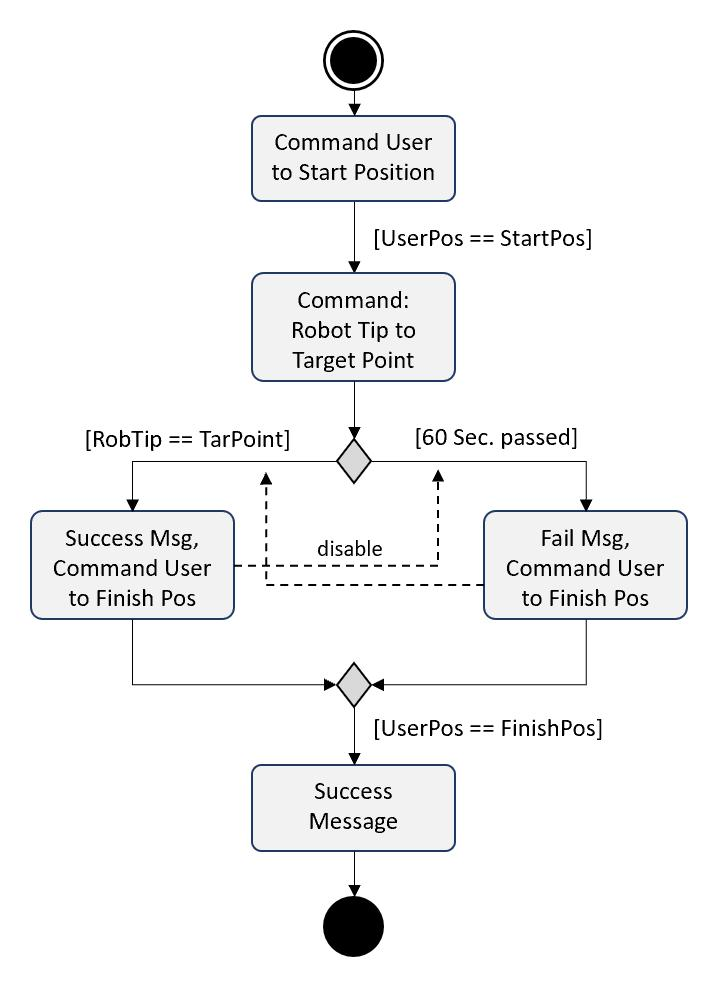
\includegraphics[width=1\linewidth]{Figures/Evaluation2_workflow}
		\caption[Evaluation 2 use case-workflow]{Evaluation 2 use case-workflow}
		\label{Fig:Evaluation2Workflow}
	\end{minipage}\hfill
	\begin{minipage}{0.55\textwidth}
		\begin{enumerate}
			\item The User should approach the robot safely by walking to the starting position.
			\item Then, the robot should be jogged into a given position in under 1 minute.
			\item The application should then display a success or failure message according to step 2.
			\item In both cases, the user should be commanded to move away into the finishing position, such that the robot can not inflict any damage.
		\end{enumerate} 
		The coordinates of the Start, Finish and Robot-Target Points were given to the experimentees. Fig.~\ref{Fig:Evaluation2Workflow} depicts one solution to the given task as a workflow diagram. 
	\end{minipage}
\end{figure}

\FloatBarrier

Each experimentee was given an explanation of the PARRHI system and syntax, and was provided a cheat sheet, which briefly summarised all commands and object definitions in the PARRHI system. The basis of their work was the same Parametrised Program template, as it was used for the PARRHI attempt in evaluation 1. The participants were asked to develop an AR application according to the Use Case definition above using the PARRHI system. After they completed their task, they were asked three questions, the answers of which are summarised below. Their work was timed and evaluated whether or not they successfully achieved the goal. I was available for questions during their attempts, but did not answer any questions regarding the core concept of the PARRHI system. 

A valid solution to the given task can be found in the Appendix A. In total it contains 23 object definitions, which reflect and build the given workflow and had to be written by the experimentees. There are multiple valid solutions to the task.

\subsection{Summary Evaluation 2}

The second evaluation has been completed by six people, five of which are mechanical engineering and one a software engineering bachelor student all aged from 20 to 25. It is important to note that no students knew anything about the PARRHI system and the parametrised program syntax beforehand, and it was their first attempt of developing with it. All students had some minor experiences with different programming languages, and about half of them are very experienced in different programming related technology stacks. None of them had any experience in Augmented Reality development.

Five out of the six students reached their goal, with the average time being 42 minutes, excluding the student who did not succeed, who took about 55 minutes while omitting the time limit during step 2. While two students did not ask any questions and worked completely unassisted, some others did not comprehend the new system as fast and needed some guidance along the way. I tried not to answer questions regarding the core concept of the Parametrised Program. Most questions answered regarded the use case's workflow.

All but one student took a chronological approach to the task. The only software engineer approaches the challenge completely different. He first counted the number of elements in each category he might need and wrote them down. In the end, he connected all elements by filling out the corresponding parameters. Most realised rather quickly, that they had to define the triggers deactivated and activate them when appropriate. In some but not all cases, the students lost the overview towards the end, since the given names of the parametrised program objects were not optimal. This resulted in confusion regarding the names of objects and occasionally misplacing some parameters.

Another common mistake was, that XML elements were placed within the wrong tags, which, of course, resulted in the PARRI system not accepting the Parametrised Program. The corresponding feedback message from the PARRHI system quickly helped them to solve the issue and reorganise their Parametrised Program.

After the students debugged their Parametrised Program within the simulated environment, I uploaded their project onto the used Microsoft HoloLens and let them test their application with the real robot.

All students were asked the same questions after they finished their assignment. The following listing displays the question and summarises the students' answers.
\begin{enumerate}
	\item \textit{"How much experience do you have with AR development and programming in general?"}\\
	All students had some basic experience with C programming. Some were very experienced in some other programming languages, but none of them ever developed an Augmented Reality application nor operated a robot. Only one of them used a head-mounted Augmented Reality device so far.
	\item \textit{"What do you think is the biggest advantage of the PARRHI system?"}\\
	All experimentees said, that they would never have been able to fulfil the given task without the PARRHI system, since they either do not know $C\#$, Unity or both. The software engineer, who had experience in Unity Game development answered, that it would have taken him much more time to achieve a similar result, even with his knowledge about Unity. Furthermore, they all liked the fact, that they saw immediate success with their first attempt of developing the AR application.
	\item \textit{What do you think is the biggest disadvantage of the PARRHI system?}\\
	Generally all students reported, that they either lost the overview (or were very close to do so) towards the end. The reason for that was the strict separation between triggers and their actions in the parametrised program.
	\\Since their use case was crafted in a way, that it was possible to succeed with the PARRHI system, none of them saw a weakness in the PARRHI system's capabilities. During the discussion, they all agreed, that it is currently impossible to solve very specific problems, which require a different kind of trigger or action, since the developer cannot define any custom object types.\\A solution to both mentioned problems will be proposed in section~\ref{Section:FutureWork}.
\end{enumerate}
 
\section{Solution to Problems Found in the Evaluation}\label{Section:SolutionToEval}
 
The evaluation found two major flaws in the current concept of the PARRHI system. Firstly, the expermimentees lost the overview of their own parametrised program. Secondly, the possible use cases are limited by PARRHI's predefined capabilities.

\subsection{Solution to Problem 1: Overview and Program Complexity}
This problem might be solvable in two distinct but not exclusive ways.

The discussion with the experimentees from evaluation 2 brought up, that a simple re-organisation of the parametrised program's structure could help to increase the overview. Namely, the separation of triggers and their corresponding actions in combination with the name referencing confused the developers, when their program grew in length.

By allowing actions and triggers to be defined underneath the same XML-parent element, the logical workflow could be represented in the program much better. Furthermore, adding the possibility to define "inline actions" would help to reduce the number of names (and with that the confusion) within a program.

Most of the time, one action was exclusively triggered by one trigger. This one to one relationship could be referenced implicitly by defining the action as an XML-child of the trigger. As shown in the example below. A trigger would then invoke all implicitly referenced actions in addition to the ones defined with the \code{actions} parameter.

These implicitly referenced actions do not need a name parameter since their execution is defined by their parent trigger.

\begin{lstlisting}
<!-- Define Trigger -->
<DistanceTrigger name="DTrigger" point1="..." point2="..." distance="15" actions="...">
	<!-- Define Action -->
	<ChangeUITextAction text="You have reached your target successfully!"/>
</DistanceTrigger>
\end{lstlisting}

Another possible solution to reduce the confusion and complexity within the parametrised program would be a graphical editor, which generates the XML document. The syntax defined in the parametrised program is an almost perfect fit for UML activity diagrams (for reference, see Fig.~\ref{Fig:Evaluation2Workflow}.).

\subsection{Solution to Problem 2: PARRHI's Limitations}

With the PARRHI system the developer can only perform actions, which are directly supported by the different types of actions. Whenever an action, which is not available in the PARRHI system, should be performed, the system reaches its limits. The same is true if the application should display holograms in different shapes than spheres and cylinders.

This problem could be overcome by allowing the developer to define custom implementations of certain components within the parametrised program. In the simplest case, this implementation could be provided in a specific $C\#$ source code file. The developer would get access to all parameters provided by the PARRHI system, and would also be able to reference objects defined within the parametrised program.

This way, the developer could setup and solve the simple parts within the parametrised program with the supplied object types, and implement everything else on their own. For example, if the developer needs a very specific trigger to be defined, they could achieve that, by directly implementing them in source code. The developer would still not care about any AR functionalities and can still focus on his domain knowledge. 

The defined custom components could then be used in the parametrised program as any other type of trigger, provided they are implemented with the correct properties. 

The real-life usage could be, that developers continuously extend their custom implementations, and use them like normal elements in the parametrised program. In larger companies, one software engineer could take over the task of implementing these specific functionalities, and less skilled or specialised developers could use these custom elements in their parametrised program.

 
 
 
 
 
 
 
 
 
 
 
 
 
 
 
 
 
 